\documentclass[../TAU.tex]{subfiles}



\theoremstyle{plain}
\newtheorem{theor}{\bf Теорема \thetheor}
\newtheorem{statement}{\bf Утверждение \thestatement}
%%%%%%%%%%%%%%%%%%%%%%%%%%%%%%%%%%%%%%%%%%%%%%%%%%%%%%%%%%%%%%%%%%%%%%%%%%
%%%%%%%%%%%%%%%%%%%%%%%%%%%%%%%%%%%%%%%%%%%%%%%%%%%%%%%%%%%%%%%%%%%%%%%%%%
\theoremstyle{definition}
\newtheorem{defi}{\bf Определение \thedefi}
\newtheorem{task}{\bf Задача  \thetask}
\theoremstyle{remark}
\newtheorem{remark}{\bf Замечание \theremark}
\newtheorem{examp}{\bf Пример}
\theoremstyle{plain}
%%%%%%%%%%%%%%%%%%%%%%%%%%%%%%%%%%%%%%%%%%%%%%%%%%%%%%%%%%%%%%%%%%%%%%%%%%
\newcommand{\eref}[1]{(\ref{#1})}
\newcommand{\const}{\mathop{\mathrm{const}}\nolimits}
\newcommand{\col}{\mathop{\mathrm{col}}\nolimits}
\newcommand{\diag}{\mathop{\mathrm{diag}}\nolimits}
\newcommand{\rank}{\mathop{\mathrm{rank}}\nolimits}
\newcommand{\spec}{\mathop{\mathrm{spec}}\nolimits}
\newcommand{\rang}{\mathop{\mathrm{rang}}\nolimits}
\newcommand{\RE}{\mathop{\mathrm{Re}}\nolimits}
\newcommand{\IM}{\mathop{\mathrm{Im}}\nolimits}
\newcommand{\cnt}[1]{\overline{#1}}
\newcommand{\BF}[1]{\mathbb{#1}}
\newcommand{\IT}[1]{\mathcal{#1}}


% these will be used later in the title page
\title[Основы теории автоматического управления]{Основы теории автоматического управления}
\author{ Капалин И.В.}


\begin{document}

\section{Main}




\begin{center}
{\small НИТУ МИСиС\\
Кафедра инженерной кибернетики
}
\end{center}

\vspace{1cm}

\begin{center}
Курс\\
{\LARGE Основы теории автоматического управления (ТАУ)}
\end{center}
\vspace{1cm}

\begin{flushright}
{\small
Лектор:\\
Капалин Иван Владимирович\\
к.ф.-м.н., доцент
}
\end{flushright}

\begin{center}
2013     год\\
Москва
\end{center}





\begin{center}
{\LARGE
Лекция №1\\
Предмет ТАУ. Основные понятия, структура и классификация систем автоматического управления}
\end{center}





\section{Введение}

\begin{center}
Процессы управления\\ [4pt]
\begin{tabular}{|p{5.5cm}|p{5.5cm}|}
  % after \\: \hline or \cline{col1-col2} \cline{col3-col4} ...
  \hline
  В живой природе & В неживой природе \\ [4pt]
  \hline
  Естественный отбор & Наведение на цель орудия \\
  \hline
  терморегуляция у животных & поддержание температуры в печи\\
  \hline
  поддержание равновесия животными & поддержание равновесия робота\\
  \hline
  увеличение рождаемости в стране & поддержание скорости на моторе\\
  \hline
  уничтожение клеток определенного типа (вирусных, инфекционных и т.п.)& поддержание фиксированной высоты летального аппарата\\
  \hline
  повышение работоспособности работников предприятия & выполнение траектории ракетой\\
  \hline
\end{tabular}
\end{center}




\section{Введение}

Общее характеристики всех процессов управления:
\begin{enumerate}
\item Прием информации (камера, глаза, датчики давления, скорости, положения и т.п., общение)\\
\item Хранение информации (память животных, память на носителях (USB, HDD, CD, DVD))\\
\item Преобразование информации (анализ рынка, те или иные вычисления)\\
\item Выработка управляющего воздействия (подача напряжения на мотор, передача указаний подчиненным, поворот руля)
\end{enumerate}

Научное направление занимающееся изучение процессов управления, называется кибернетикой. Основано Н. Винером в конце 40х годов 20 века.

В этом курсе мы будем заниматься только процессами управления в {\it неживой} природе, т.е. теорией автоматического управления.




\section{Исходные положения ТАУ. Термины}

{\it Управлением} называется целенаправленное воздействие на объект или устройств. Управление может быть автоматическим, т.е. без участия человека, либо ручным.\\

{\it Устройство}, которым нужно и можно управлять, называют объектом управления (ОУ).\\

{\it Целью управления} ОУ является поддержание {\it заданного режима}, т.е. изменение какого-либо параметра ОУ по заданному закону (например, температура в холодильнике должна быть фиксированной). \\

Такой параметр называют {\it управляемой или выходной переменной}.\\

{\it Устройство управления (УУ)} и ОУ вместе называют системой автоматического управления (САУ).\\




\section{Исходные положения ТАУ. Структурная схема}

\begin{figure}
\epsfig{file=./fig/SAU_scheme.pdf,width=80mm}
\end{figure}

На структурной схеме САУ: $y$ --- выходная переменная; $g$ --- задающее воздействие (иногда изображается как выход задающего устройства); $f$ --- возмущение, действующее на ОУ и, возможно, на УУ; $u$ --- управление (управляющее воздействие) . Канал связи, по которому поступает информации в УУ о состоянии ОУ, называется {\it обратной связью} (feedback). В САУ обратная связь может отсутствовать.



\section{Исходные положения ТАУ. Понятие устойчивости}

ОУ в зависимости от входных воздействий бывают устойчивые, нейтральные и неустойчивые. Например, пусть при постоянных $u = u_0, f = f_0$ на выходе $y = y_0$. Положим, что на какое-то время $T$ значение $u$ и $f$ изменились, а затем вернулись к исходным значениям. Тогда ОУ
\begin{enumerate}
\item устойчивый, если при $t \rightarrow \infty$ выход $y \rightarrow y_0$. \\
Например, холодильник, генератор напряжение, маятник, унитаз;\\
\item нейтральный, если при $t \rightarrow \infty$ выход $y \rightarrow y_1$ и $y_1\neq y_0$. \\
Например, резервуар с водой\\
\item неустойчивый в противном случае.\\
Самолет с обратной стреловидностью, обратный (перевернутый) маятник.
\end{enumerate}




\section{Принципы управления (программное, компенсации)}

\begin{enumerate}
\item {\it Программное управление.}\\
Управление $u$ выбирается в виде некоторой функции времени $u = u(t)$.
\begin{center}
\epsfig{file=./fig/program.pdf,width=80mm}
\end{center}
Условием применимости этого принципа является полная информация об ОУ, его устойчивость и отсутствие существенных неизвестных возмущений.
\item {\it Принцип компенсации.}\\
Управление $u$ вырабатывается на основе информации о возмущении, что служит и ограничением применимости принципа. При этом можно выделить методы при прямом и косвенном измерении возмущения.

\end{enumerate}




\section{Принципы управления. Обратная связь}

\begin{enumerate}
\setcounter{enumi}{2}
\item {\it Принцип обратной связи.}\\
Один из самых универсальных методов управления, т.к. не требует информации о возмущениях. А в его специальных модификациях условие устойчивости исходного объекта не обязательно.
\begin{center}
\epsfig{file=./fig/feedback.pdf,width=70mm}
\end{center}
Недостатки: невозможность полной компенсации возмущения, в прямом применении может сделать ОУ неустойчивым.
\item {\it Принцип комбинированного управления.}\\
Совместное использование вышеперечисленных принципов управления.
\end{enumerate}






\section{Структура АСУ}

\begin{center}
\epsfig{file=./fig/SAU_structure.pdf,width=90mm}
\end{center}

На схеме: ЧЭ, чувствительный элемент, измеряющий возмущения (не всегда присутствует) и выход $y$; УПУ, усилительно-преобразовательное устройство, вырабатывающее управление $u$ на основе задающего воздействия $g$ и, возможно, измерения $f$; ИУ, исполнительное устройство, которое непосредственно воздействует на ОУ; СУ, сравнительное устройство, вычисляющее отклонение $e$; ЗУ, задающее устройство, вырабатывающее задающее воздействие $g$.




\section{Классификация САУ}

САУ различают по:
\begin{enumerate}
\item наличию обратной связи: замкнутые (с обратной связью) и разомкнутые (без обратной связи);
\item виду задающего воздействия $g$:
\begin{enumerate}
\item системы стабилизации: $g=const$;
\item системы программного управления: $g=g(t)$ --- заданная функция;
\item системы слежения (следящие системы): задающее воздействие определяется внешними факторами (например, радиолокация).
\end{enumerate}
\item способу использования текущей информации:
\begin{enumerate}
\item неадаптивные, т.е.  те, в которых текущая информация используется {\it только} для выработки управляющего воздействия;
\item адаптивные, т.е. те, в которых текущая информация используется еще и для изменения алгоритма управления или его параметров;
\end{enumerate}
\item виду сигналов в САУ: дискретные (если есть сигналы квантованные по уровню/времени) и непрерывные (только непрерывные сигналы);
\end{enumerate}




\section{Классификация САУ}
\begin{enumerate}
\setcounter{enumi}{4}
\item уравнениям, которыми описывается  система управления: линейные или нелинейные;
\item характеру внешних (задающих и возмущающих) воздействий:
\begin{enumerate}
  \item детерминированные: нет случайных воздействий;
  \item стохастические: есть случайные воздействия;
\end{enumerate}

\end{enumerate}



% До этого на доске разобрал на примере маятника типовой закон управления u = k_p * e


\section{Типовые законы управления. Применения ПД-закона (для маятника)}

\begin{center}
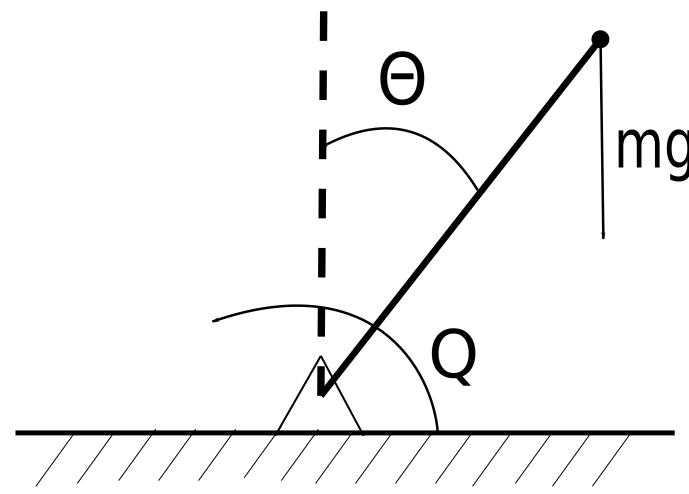
\epsfig{file=./fig/pendulum.pdf,width=40mm}
\end{center}

Уравнение, описывающее перевернутый (обратный) маятник в окрестности $\Theta=0$ имеет вид
\begin{equation}\label{EQ1}
J\ddot\Theta = -Q+mgl\Theta,
\end{equation}
где $\Theta$ --- угол отклонения от вертикальной оси, $Q$ --- вращательный момент, создаваемый мотором, $m$ --- масса маятника, $l$ --- длина подвеса
маятника, $J = ml^2$ --- момент инерции маятника, $g$ --- ускорение свободного падения.




\section{Типовые законы управления. Пример ПД-закона}

В нормальной форме уравнение \eref{EQ1} имеет вид
\begin{equation}\label{EQ1NORM}
\begin{cases}
\dot x = Ax + bu,\\
y = c x,
\end{cases}
\end{equation}
где $x = (x_1\quad x_2)^T = ( \Theta\quad \dot\Theta)^T$ --- вектор состояния системы, $A =\begin{pmatrix}0 & 1\\ \omega^2& 0\end{pmatrix}$,$b = (0\quad 1)^T$, $c = (1\quad0)$,$\omega = \sqrt{\frac{g}{l}}$, $u = -\frac{Q}{J}$ --- управление (вход) и $y = cx = x_1 = \Theta$ --- регулируемый (или измеряемый) параметр.

Цель управления: стабилизировать маятник в положении $\Theta_0 = 0$ (задающее воздействие $g = 0$).

Используем принцип обратной связи и ПД-закон для решения задачи. Тогда


$$
u = k_п e + k_д \dot e,
$$
где $e$ --- отклонение от заданного режима, т.е. $e = \Theta_0 - y = -y = -x_1$, $k_п$ и $k_д$ --- коэффициенты, подлежащие определению.




\section{Типовые законы управления. Пример ПД-закона}

Учитывая первое уравнение $\dot x_1 = x_2$ в системе \eref{EQ1NORM}, получим
$$
u = - k_п x_1 - k_д \dot x_1 = - (k_п\quad k_д) \begin{pmatrix}x_1 \\ x_2\end{pmatrix}.
$$

Подставляя это управление в \eref{EQ1NORM}, получим систему
\begin{equation}\label{EQ2}
\begin{cases}
\dot x = A_kx,\\
y = c x,
\end{cases}
\end{equation}
где $A_k = A - b(k_п\quad k_д)=\begin{pmatrix}0 & 1\\ \omega^2 - k_п& - k_д\end{pmatrix}$.

Остается выбрать коэффициенты ПД-закона, исходя из устойчивости системы \eref{EQ2}. Причем добьемся того, чтобы в установившемся режиме не было колебаний. Это эквивалентно тому, что у характеристического полинома системы \eref{EQ2} есть только действительные отрицательные корни.




\section{Типовые законы управления. Пример ПД-закона}
В данном случае характеристический полином замкнутой системы имеет вид
$$
\gamma(s) = \det (Is-A_k) = s^2+ k_дs+(k_п-\omega^2).
$$
Тогда выбрав $k_д$ и $k_п$ так, что $\gamma(s)$ имеет только отрицательные корни, получим устойчивую САУ и тем самым стабилизируем маятник в положении $\Theta_0 = 0$.

\begin{figure}
\centering
\epsfig{file=./fig/feedback_pendulum.pdf,width=60mm}
\centering
\caption{Структурная схема САУ перевернутого маятника}
\end{figure}
На схеме ОУ (маятник с мотором) описан с помощью ОДУ \eref{EQ1}, УУ (компьютер/контроллер устанавливающий желаемый момент вращения Q) описывается оператором $R = k_п+k_д\frac{d}{dt}$ и реализует ПД-закон управления.





\end{document}
